% Formatting of listings
\lstset{language=C, frame=L, basicstyle=\footnotesize,%\sffamily,
	keywordstyle=\bfseries, showstringspaces=false, xleftmargin=\parindent, numbers=none, numberstyle=\tiny, stepnumber=2, numbersep=5pt}
\newpage
\section{Реализация}
\label{sec:Design}
\subsection{Программные средства реализации}
Для разработки программной части приложения использовался высокоуровневый язык программирования Python версии 3.9.18. Программирование осуществлялось в интегрированной среде разработки PyCharm Community 2023.3.4~\cite{pycharm}.
\vspace{2em}
\subsection{Реализация компонентов приложения}
Описать работу каждого модуля, входные и выходные данные, вставить код.


\vspace{2em}
\subsection{Реализация пользовательского интерфейса}
Реализация пользовательского интерфейса осуществлялась на основе разработанных макетов. Реализованы окна главного меню, разметки песен и визуализации результатов. В качестве основы разработки интерфейса использовалась библиотека tkinter~\cite{tkinter}.

\begin{figure}
    \centering
    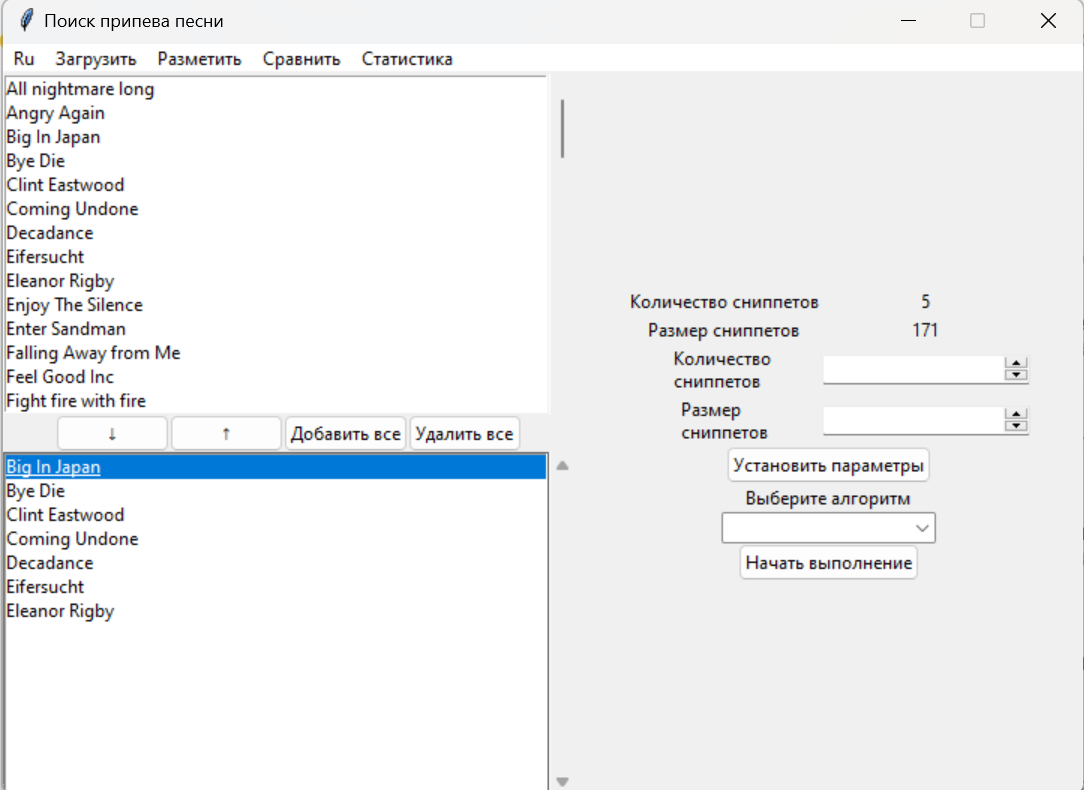
\includegraphics[width=1\linewidth]{pictures/Главный_скрин.png}
    \caption{Окно главного меню}
    \label{fig:Главный_скрин}
\end{figure}

На рисунке~\ref{fig:Главный_скрин} представлено главное окно приложения. Оно содержит два списка песен, два поля для просмотра параметров песни, два поля для ввода числовых значений, кнопку для сохранения введённых параметров, выпадающий список с выбором алгоритма классификации и кнопку начала работы. Кроме того, главное окно имеет верхнее меню, в котором можно сменить язык с русского на английский, загрузить тексты песен в приложение, открыть окно разметки и открыть окно визуализации результатов.

\begin{figure}
    \centering
    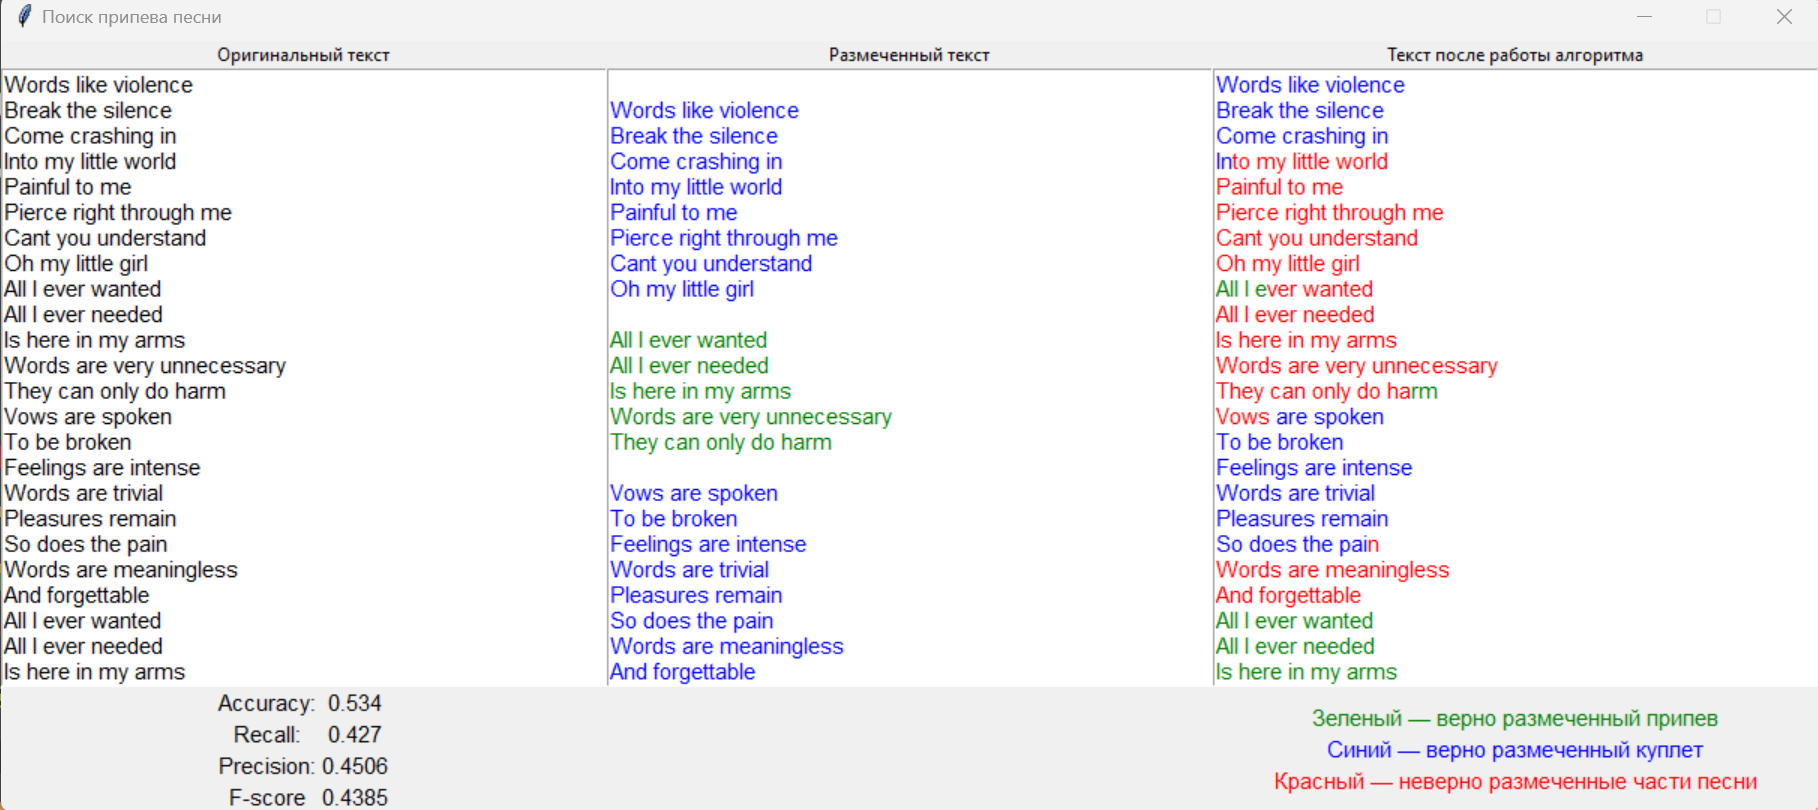
\includegraphics[width=1\linewidth]{pictures/Результаты_скрин.png}
    \caption{Окно визуализации результатов}
    \label{fig:Результаты_скрин}
\end{figure}

На рисунке~\ref{fig:Результаты_скрин} представлено окно визуализации результатов. Оно содержит три текстовых поля с текстом песни, метрики, такие как accuracy, precision, recall и F-score.